
% Default to the notebook output style

    


% Inherit from the specified cell style.




    
\documentclass[11pt]{article}

    
    
    \usepackage[T1]{fontenc}
    % Nicer default font (+ math font) than Computer Modern for most use cases
    \usepackage{mathpazo}

    % Basic figure setup, for now with no caption control since it's done
    % automatically by Pandoc (which extracts ![](path) syntax from Markdown).
    \usepackage{graphicx}
    \usepackage{float}
    % We will generate all images so they have a width \maxwidth. This means
    % that they will get their normal width if they fit onto the page, but
    % are scaled down if they would overflow the margins.
    \makeatletter
    \def\maxwidth{\ifdim\Gin@nat@width>\linewidth\linewidth
    \else\Gin@nat@width\fi}
    \makeatother
    \let\Oldincludegraphics\includegraphics
    % Set max figure width to be 80% of text width, for now hardcoded.
    \renewcommand{\includegraphics}[1]{\Oldincludegraphics[width=.8\maxwidth]{#1}}
    % Ensure that by default, figures have no caption (until we provide a
    % proper Figure object with a Caption API and a way to capture that
    % in the conversion process - todo).
    \usepackage{caption}
    \DeclareCaptionLabelFormat{nolabel}{}
    \captionsetup{labelformat=nolabel}

    \usepackage{adjustbox} % Used to constrain images to a maximum size 
    \usepackage{xcolor} % Allow colors to be defined
    \usepackage{enumerate} % Needed for markdown enumerations to work
    \usepackage{geometry} % Used to adjust the document margins
    \usepackage{amsmath} % Equations
    \usepackage{amssymb} % Equations
    \usepackage{textcomp} % defines textquotesingle
    % Hack from http://tex.stackexchange.com/a/47451/13684:
    \AtBeginDocument{%
        \def\PYZsq{\textquotesingle}% Upright quotes in Pygmentized code
    }
    \usepackage{upquote} % Upright quotes for verbatim code
    \usepackage{eurosym} % defines \euro
    \usepackage[mathletters]{ucs} % Extended unicode (utf-8) support
    \usepackage[utf8x]{inputenc} % Allow utf-8 characters in the tex document
    \usepackage{fancyvrb} % verbatim replacement that allows latex
    \usepackage{grffile} % extends the file name processing of package graphics 
                         % to support a larger range 
    % The hyperref package gives us a pdf with properly built
    % internal navigation ('pdf bookmarks' for the table of contents,
    % internal cross-reference links, web links for URLs, etc.)
    \usepackage{hyperref}
    \usepackage{longtable} % longtable support required by pandoc >1.10
    \usepackage{booktabs}  % table support for pandoc > 1.12.2
    \usepackage[inline]{enumitem} % IRkernel/repr support (it uses the enumerate* environment)
    \usepackage[normalem]{ulem} % ulem is needed to support strikethroughs (\sout)
                                % normalem makes italics be italics, not underlines
    \usepackage{mathrsfs}
    

    
    
    % Colors for the hyperref package
    \definecolor{urlcolor}{rgb}{0,.145,.698}
    \definecolor{linkcolor}{rgb}{.71,0.21,0.01}
    \definecolor{citecolor}{rgb}{.12,.54,.11}

    % ANSI colors
    \definecolor{ansi-black}{HTML}{3E424D}
    \definecolor{ansi-black-intense}{HTML}{282C36}
    \definecolor{ansi-red}{HTML}{E75C58}
    \definecolor{ansi-red-intense}{HTML}{B22B31}
    \definecolor{ansi-green}{HTML}{00A250}
    \definecolor{ansi-green-intense}{HTML}{007427}
    \definecolor{ansi-yellow}{HTML}{DDB62B}
    \definecolor{ansi-yellow-intense}{HTML}{B27D12}
    \definecolor{ansi-blue}{HTML}{208FFB}
    \definecolor{ansi-blue-intense}{HTML}{0065CA}
    \definecolor{ansi-magenta}{HTML}{D160C4}
    \definecolor{ansi-magenta-intense}{HTML}{A03196}
    \definecolor{ansi-cyan}{HTML}{60C6C8}
    \definecolor{ansi-cyan-intense}{HTML}{258F8F}
    \definecolor{ansi-white}{HTML}{C5C1B4}
    \definecolor{ansi-white-intense}{HTML}{A1A6B2}
    \definecolor{ansi-default-inverse-fg}{HTML}{FFFFFF}
    \definecolor{ansi-default-inverse-bg}{HTML}{000000}

    % commands and environments needed by pandoc snippets
    % extracted from the output of `pandoc -s`
    \providecommand{\tightlist}{%
      \setlength{\itemsep}{0pt}\setlength{\parskip}{0pt}}
    \DefineVerbatimEnvironment{Highlighting}{Verbatim}{commandchars=\\\{\}}
    % Add ',fontsize=\small' for more characters per line
    \newenvironment{Shaded}{}{}
    \newcommand{\KeywordTok}[1]{\textcolor[rgb]{0.00,0.44,0.13}{\textbf{{#1}}}}
    \newcommand{\DataTypeTok}[1]{\textcolor[rgb]{0.56,0.13,0.00}{{#1}}}
    \newcommand{\DecValTok}[1]{\textcolor[rgb]{0.25,0.63,0.44}{{#1}}}
    \newcommand{\BaseNTok}[1]{\textcolor[rgb]{0.25,0.63,0.44}{{#1}}}
    \newcommand{\FloatTok}[1]{\textcolor[rgb]{0.25,0.63,0.44}{{#1}}}
    \newcommand{\CharTok}[1]{\textcolor[rgb]{0.25,0.44,0.63}{{#1}}}
    \newcommand{\StringTok}[1]{\textcolor[rgb]{0.25,0.44,0.63}{{#1}}}
    \newcommand{\CommentTok}[1]{\textcolor[rgb]{0.38,0.63,0.69}{\textit{{#1}}}}
    \newcommand{\OtherTok}[1]{\textcolor[rgb]{0.00,0.44,0.13}{{#1}}}
    \newcommand{\AlertTok}[1]{\textcolor[rgb]{1.00,0.00,0.00}{\textbf{{#1}}}}
    \newcommand{\FunctionTok}[1]{\textcolor[rgb]{0.02,0.16,0.49}{{#1}}}
    \newcommand{\RegionMarkerTok}[1]{{#1}}
    \newcommand{\ErrorTok}[1]{\textcolor[rgb]{1.00,0.00,0.00}{\textbf{{#1}}}}
    \newcommand{\NormalTok}[1]{{#1}}
    
    % Additional commands for more recent versions of Pandoc
    \newcommand{\ConstantTok}[1]{\textcolor[rgb]{0.53,0.00,0.00}{{#1}}}
    \newcommand{\SpecialCharTok}[1]{\textcolor[rgb]{0.25,0.44,0.63}{{#1}}}
    \newcommand{\VerbatimStringTok}[1]{\textcolor[rgb]{0.25,0.44,0.63}{{#1}}}
    \newcommand{\SpecialStringTok}[1]{\textcolor[rgb]{0.73,0.40,0.53}{{#1}}}
    \newcommand{\ImportTok}[1]{{#1}}
    \newcommand{\DocumentationTok}[1]{\textcolor[rgb]{0.73,0.13,0.13}{\textit{{#1}}}}
    \newcommand{\AnnotationTok}[1]{\textcolor[rgb]{0.38,0.63,0.69}{\textbf{\textit{{#1}}}}}
    \newcommand{\CommentVarTok}[1]{\textcolor[rgb]{0.38,0.63,0.69}{\textbf{\textit{{#1}}}}}
    \newcommand{\VariableTok}[1]{\textcolor[rgb]{0.10,0.09,0.49}{{#1}}}
    \newcommand{\ControlFlowTok}[1]{\textcolor[rgb]{0.00,0.44,0.13}{\textbf{{#1}}}}
    \newcommand{\OperatorTok}[1]{\textcolor[rgb]{0.40,0.40,0.40}{{#1}}}
    \newcommand{\BuiltInTok}[1]{{#1}}
    \newcommand{\ExtensionTok}[1]{{#1}}
    \newcommand{\PreprocessorTok}[1]{\textcolor[rgb]{0.74,0.48,0.00}{{#1}}}
    \newcommand{\AttributeTok}[1]{\textcolor[rgb]{0.49,0.56,0.16}{{#1}}}
    \newcommand{\InformationTok}[1]{\textcolor[rgb]{0.38,0.63,0.69}{\textbf{\textit{{#1}}}}}
    \newcommand{\WarningTok}[1]{\textcolor[rgb]{0.38,0.63,0.69}{\textbf{\textit{{#1}}}}}
    
    
    % Define a nice break command that doesn't care if a line doesn't already
    % exist.
    \def\br{\hspace*{\fill} \\* }
    % Math Jax compatibility definitions
    \def\gt{>}
    \def\lt{<}
    \let\Oldtex\TeX
    \let\Oldlatex\LaTeX
    \renewcommand{\TeX}{\textrm{\Oldtex}}
    \renewcommand{\LaTeX}{\textrm{\Oldlatex}}
    % Document parameters
    % Document title
    \title{Assignment 4}
    \author{Jiarong Ye}
    
    
    
    

    % Pygments definitions
    
\makeatletter
\def\PY@reset{\let\PY@it=\relax \let\PY@bf=\relax%
    \let\PY@ul=\relax \let\PY@tc=\relax%
    \let\PY@bc=\relax \let\PY@ff=\relax}
\def\PY@tok#1{\csname PY@tok@#1\endcsname}
\def\PY@toks#1+{\ifx\relax#1\empty\else%
    \PY@tok{#1}\expandafter\PY@toks\fi}
\def\PY@do#1{\PY@bc{\PY@tc{\PY@ul{%
    \PY@it{\PY@bf{\PY@ff{#1}}}}}}}
\def\PY#1#2{\PY@reset\PY@toks#1+\relax+\PY@do{#2}}

\expandafter\def\csname PY@tok@w\endcsname{\def\PY@tc##1{\textcolor[rgb]{0.73,0.73,0.73}{##1}}}
\expandafter\def\csname PY@tok@c\endcsname{\let\PY@it=\textit\def\PY@tc##1{\textcolor[rgb]{0.25,0.50,0.50}{##1}}}
\expandafter\def\csname PY@tok@cp\endcsname{\def\PY@tc##1{\textcolor[rgb]{0.74,0.48,0.00}{##1}}}
\expandafter\def\csname PY@tok@k\endcsname{\let\PY@bf=\textbf\def\PY@tc##1{\textcolor[rgb]{0.00,0.50,0.00}{##1}}}
\expandafter\def\csname PY@tok@kp\endcsname{\def\PY@tc##1{\textcolor[rgb]{0.00,0.50,0.00}{##1}}}
\expandafter\def\csname PY@tok@kt\endcsname{\def\PY@tc##1{\textcolor[rgb]{0.69,0.00,0.25}{##1}}}
\expandafter\def\csname PY@tok@o\endcsname{\def\PY@tc##1{\textcolor[rgb]{0.40,0.40,0.40}{##1}}}
\expandafter\def\csname PY@tok@ow\endcsname{\let\PY@bf=\textbf\def\PY@tc##1{\textcolor[rgb]{0.67,0.13,1.00}{##1}}}
\expandafter\def\csname PY@tok@nb\endcsname{\def\PY@tc##1{\textcolor[rgb]{0.00,0.50,0.00}{##1}}}
\expandafter\def\csname PY@tok@nf\endcsname{\def\PY@tc##1{\textcolor[rgb]{0.00,0.00,1.00}{##1}}}
\expandafter\def\csname PY@tok@nc\endcsname{\let\PY@bf=\textbf\def\PY@tc##1{\textcolor[rgb]{0.00,0.00,1.00}{##1}}}
\expandafter\def\csname PY@tok@nn\endcsname{\let\PY@bf=\textbf\def\PY@tc##1{\textcolor[rgb]{0.00,0.00,1.00}{##1}}}
\expandafter\def\csname PY@tok@ne\endcsname{\let\PY@bf=\textbf\def\PY@tc##1{\textcolor[rgb]{0.82,0.25,0.23}{##1}}}
\expandafter\def\csname PY@tok@nv\endcsname{\def\PY@tc##1{\textcolor[rgb]{0.10,0.09,0.49}{##1}}}
\expandafter\def\csname PY@tok@no\endcsname{\def\PY@tc##1{\textcolor[rgb]{0.53,0.00,0.00}{##1}}}
\expandafter\def\csname PY@tok@nl\endcsname{\def\PY@tc##1{\textcolor[rgb]{0.63,0.63,0.00}{##1}}}
\expandafter\def\csname PY@tok@ni\endcsname{\let\PY@bf=\textbf\def\PY@tc##1{\textcolor[rgb]{0.60,0.60,0.60}{##1}}}
\expandafter\def\csname PY@tok@na\endcsname{\def\PY@tc##1{\textcolor[rgb]{0.49,0.56,0.16}{##1}}}
\expandafter\def\csname PY@tok@nt\endcsname{\let\PY@bf=\textbf\def\PY@tc##1{\textcolor[rgb]{0.00,0.50,0.00}{##1}}}
\expandafter\def\csname PY@tok@nd\endcsname{\def\PY@tc##1{\textcolor[rgb]{0.67,0.13,1.00}{##1}}}
\expandafter\def\csname PY@tok@s\endcsname{\def\PY@tc##1{\textcolor[rgb]{0.73,0.13,0.13}{##1}}}
\expandafter\def\csname PY@tok@sd\endcsname{\let\PY@it=\textit\def\PY@tc##1{\textcolor[rgb]{0.73,0.13,0.13}{##1}}}
\expandafter\def\csname PY@tok@si\endcsname{\let\PY@bf=\textbf\def\PY@tc##1{\textcolor[rgb]{0.73,0.40,0.53}{##1}}}
\expandafter\def\csname PY@tok@se\endcsname{\let\PY@bf=\textbf\def\PY@tc##1{\textcolor[rgb]{0.73,0.40,0.13}{##1}}}
\expandafter\def\csname PY@tok@sr\endcsname{\def\PY@tc##1{\textcolor[rgb]{0.73,0.40,0.53}{##1}}}
\expandafter\def\csname PY@tok@ss\endcsname{\def\PY@tc##1{\textcolor[rgb]{0.10,0.09,0.49}{##1}}}
\expandafter\def\csname PY@tok@sx\endcsname{\def\PY@tc##1{\textcolor[rgb]{0.00,0.50,0.00}{##1}}}
\expandafter\def\csname PY@tok@m\endcsname{\def\PY@tc##1{\textcolor[rgb]{0.40,0.40,0.40}{##1}}}
\expandafter\def\csname PY@tok@gh\endcsname{\let\PY@bf=\textbf\def\PY@tc##1{\textcolor[rgb]{0.00,0.00,0.50}{##1}}}
\expandafter\def\csname PY@tok@gu\endcsname{\let\PY@bf=\textbf\def\PY@tc##1{\textcolor[rgb]{0.50,0.00,0.50}{##1}}}
\expandafter\def\csname PY@tok@gd\endcsname{\def\PY@tc##1{\textcolor[rgb]{0.63,0.00,0.00}{##1}}}
\expandafter\def\csname PY@tok@gi\endcsname{\def\PY@tc##1{\textcolor[rgb]{0.00,0.63,0.00}{##1}}}
\expandafter\def\csname PY@tok@gr\endcsname{\def\PY@tc##1{\textcolor[rgb]{1.00,0.00,0.00}{##1}}}
\expandafter\def\csname PY@tok@ge\endcsname{\let\PY@it=\textit}
\expandafter\def\csname PY@tok@gs\endcsname{\let\PY@bf=\textbf}
\expandafter\def\csname PY@tok@gp\endcsname{\let\PY@bf=\textbf\def\PY@tc##1{\textcolor[rgb]{0.00,0.00,0.50}{##1}}}
\expandafter\def\csname PY@tok@go\endcsname{\def\PY@tc##1{\textcolor[rgb]{0.53,0.53,0.53}{##1}}}
\expandafter\def\csname PY@tok@gt\endcsname{\def\PY@tc##1{\textcolor[rgb]{0.00,0.27,0.87}{##1}}}
\expandafter\def\csname PY@tok@err\endcsname{\def\PY@bc##1{\setlength{\fboxsep}{0pt}\fcolorbox[rgb]{1.00,0.00,0.00}{1,1,1}{\strut ##1}}}
\expandafter\def\csname PY@tok@kc\endcsname{\let\PY@bf=\textbf\def\PY@tc##1{\textcolor[rgb]{0.00,0.50,0.00}{##1}}}
\expandafter\def\csname PY@tok@kd\endcsname{\let\PY@bf=\textbf\def\PY@tc##1{\textcolor[rgb]{0.00,0.50,0.00}{##1}}}
\expandafter\def\csname PY@tok@kn\endcsname{\let\PY@bf=\textbf\def\PY@tc##1{\textcolor[rgb]{0.00,0.50,0.00}{##1}}}
\expandafter\def\csname PY@tok@kr\endcsname{\let\PY@bf=\textbf\def\PY@tc##1{\textcolor[rgb]{0.00,0.50,0.00}{##1}}}
\expandafter\def\csname PY@tok@bp\endcsname{\def\PY@tc##1{\textcolor[rgb]{0.00,0.50,0.00}{##1}}}
\expandafter\def\csname PY@tok@fm\endcsname{\def\PY@tc##1{\textcolor[rgb]{0.00,0.00,1.00}{##1}}}
\expandafter\def\csname PY@tok@vc\endcsname{\def\PY@tc##1{\textcolor[rgb]{0.10,0.09,0.49}{##1}}}
\expandafter\def\csname PY@tok@vg\endcsname{\def\PY@tc##1{\textcolor[rgb]{0.10,0.09,0.49}{##1}}}
\expandafter\def\csname PY@tok@vi\endcsname{\def\PY@tc##1{\textcolor[rgb]{0.10,0.09,0.49}{##1}}}
\expandafter\def\csname PY@tok@vm\endcsname{\def\PY@tc##1{\textcolor[rgb]{0.10,0.09,0.49}{##1}}}
\expandafter\def\csname PY@tok@sa\endcsname{\def\PY@tc##1{\textcolor[rgb]{0.73,0.13,0.13}{##1}}}
\expandafter\def\csname PY@tok@sb\endcsname{\def\PY@tc##1{\textcolor[rgb]{0.73,0.13,0.13}{##1}}}
\expandafter\def\csname PY@tok@sc\endcsname{\def\PY@tc##1{\textcolor[rgb]{0.73,0.13,0.13}{##1}}}
\expandafter\def\csname PY@tok@dl\endcsname{\def\PY@tc##1{\textcolor[rgb]{0.73,0.13,0.13}{##1}}}
\expandafter\def\csname PY@tok@s2\endcsname{\def\PY@tc##1{\textcolor[rgb]{0.73,0.13,0.13}{##1}}}
\expandafter\def\csname PY@tok@sh\endcsname{\def\PY@tc##1{\textcolor[rgb]{0.73,0.13,0.13}{##1}}}
\expandafter\def\csname PY@tok@s1\endcsname{\def\PY@tc##1{\textcolor[rgb]{0.73,0.13,0.13}{##1}}}
\expandafter\def\csname PY@tok@mb\endcsname{\def\PY@tc##1{\textcolor[rgb]{0.40,0.40,0.40}{##1}}}
\expandafter\def\csname PY@tok@mf\endcsname{\def\PY@tc##1{\textcolor[rgb]{0.40,0.40,0.40}{##1}}}
\expandafter\def\csname PY@tok@mh\endcsname{\def\PY@tc##1{\textcolor[rgb]{0.40,0.40,0.40}{##1}}}
\expandafter\def\csname PY@tok@mi\endcsname{\def\PY@tc##1{\textcolor[rgb]{0.40,0.40,0.40}{##1}}}
\expandafter\def\csname PY@tok@il\endcsname{\def\PY@tc##1{\textcolor[rgb]{0.40,0.40,0.40}{##1}}}
\expandafter\def\csname PY@tok@mo\endcsname{\def\PY@tc##1{\textcolor[rgb]{0.40,0.40,0.40}{##1}}}
\expandafter\def\csname PY@tok@ch\endcsname{\let\PY@it=\textit\def\PY@tc##1{\textcolor[rgb]{0.25,0.50,0.50}{##1}}}
\expandafter\def\csname PY@tok@cm\endcsname{\let\PY@it=\textit\def\PY@tc##1{\textcolor[rgb]{0.25,0.50,0.50}{##1}}}
\expandafter\def\csname PY@tok@cpf\endcsname{\let\PY@it=\textit\def\PY@tc##1{\textcolor[rgb]{0.25,0.50,0.50}{##1}}}
\expandafter\def\csname PY@tok@c1\endcsname{\let\PY@it=\textit\def\PY@tc##1{\textcolor[rgb]{0.25,0.50,0.50}{##1}}}
\expandafter\def\csname PY@tok@cs\endcsname{\let\PY@it=\textit\def\PY@tc##1{\textcolor[rgb]{0.25,0.50,0.50}{##1}}}

\def\PYZbs{\char`\\}
\def\PYZus{\char`\_}
\def\PYZob{\char`\{}
\def\PYZcb{\char`\}}
\def\PYZca{\char`\^}
\def\PYZam{\char`\&}
\def\PYZlt{\char`\<}
\def\PYZgt{\char`\>}
\def\PYZsh{\char`\#}
\def\PYZpc{\char`\%}
\def\PYZdl{\char`\$}
\def\PYZhy{\char`\-}
\def\PYZsq{\char`\'}
\def\PYZdq{\char`\"}
\def\PYZti{\char`\~}
% for compatibility with earlier versions
\def\PYZat{@}
\def\PYZlb{[}
\def\PYZrb{]}
\makeatother


    % Exact colors from NB
    \definecolor{incolor}{rgb}{0.0, 0.0, 0.5}
    \definecolor{outcolor}{rgb}{0.545, 0.0, 0.0}



    
    % Prevent overflowing lines due to hard-to-break entities
    \sloppy 
    % Setup hyperref package
    \hypersetup{
      breaklinks=true,  % so long urls are correctly broken across lines
      colorlinks=true,
      urlcolor=urlcolor,
      linkcolor=linkcolor,
      citecolor=citecolor,
      }
    % Slightly bigger margins than the latex defaults
    
    \geometry{verbose,tmargin=1in,bmargin=1in,lmargin=1in,rmargin=1in}
    
    

    \begin{document}
    
    
    \maketitle
    
    

    
    \subsection*{Import Packages}\label{import-packages}

    \begin{Verbatim}[commandchars=\\\{\}]
{\color{incolor}In [{\color{incolor}1}]:} \PY{k+kn}{import} \PY{n+nn}{pandas} \PY{k}{as} \PY{n+nn}{pd}
        \PY{k+kn}{import} \PY{n+nn}{json}
\end{Verbatim}

    \subsection*{Task 1}\label{task-1}

Insert 4 vehicles from the State College Auto Database (can be the same
ones you used in Redis) into the MongoDB. One easy way to do this is to
create a .json file from the data and then import the .json file into a
new data collection using the 'mongoimport' package as you did in HW \#3
to import the restaurant dataset.

    \begin{Verbatim}[commandchars=\\\{\}]
{\color{incolor}In [{\color{incolor}14}]:} \PY{n}{cars} \PY{o}{=} \PY{n}{pd}\PY{o}{.}\PY{n}{read\PYZus{}csv}\PY{p}{(}\PY{l+s+s1}{\PYZsq{}}\PY{l+s+s1}{cars.csv}\PY{l+s+s1}{\PYZsq{}}\PY{p}{,}\PY{n}{sep}\PY{o}{=}\PY{l+s+s1}{\PYZsq{}}\PY{l+s+s1}{,}\PY{l+s+s1}{\PYZsq{}}\PY{p}{,}\PY{n}{index\PYZus{}col}\PY{o}{=}\PY{l+m+mi}{0}\PY{p}{)}
         \PY{k}{with} \PY{n+nb}{open}\PY{p}{(}\PY{l+s+s1}{\PYZsq{}}\PY{l+s+s1}{cars.json}\PY{l+s+s1}{\PYZsq{}}\PY{p}{,} \PY{l+s+s1}{\PYZsq{}}\PY{l+s+s1}{w}\PY{l+s+s1}{\PYZsq{}}\PY{p}{)} \PY{k}{as} \PY{n}{outfile}\PY{p}{:}
             \PY{n}{cars\PYZus{}dict} \PY{o}{=} \PY{n}{cars}\PY{o}{.}\PY{n}{to\PYZus{}dict}\PY{p}{(}\PY{l+s+s1}{\PYZsq{}}\PY{l+s+s1}{index}\PY{l+s+s1}{\PYZsq{}}\PY{p}{)}
             \PY{k}{for} \PY{n}{i} \PY{o+ow}{in} \PY{n+nb}{range}\PY{p}{(}\PY{n+nb}{len}\PY{p}{(}\PY{n}{cars\PYZus{}dict}\PY{p}{)}\PY{p}{)}\PY{p}{:}
                 \PY{n}{json}\PY{o}{.}\PY{n}{dump}\PY{p}{(}\PY{n}{cars\PYZus{}dict}\PY{p}{[}\PY{n}{i}\PY{p}{]}\PY{p}{,} \PY{n}{outfile}\PY{p}{)}
\end{Verbatim}

    \begin{Verbatim}[commandchars=\\\{\}]
{\color{incolor}In [{\color{incolor}15}]:} \PY{o}{!} mongoimport \PYZhy{}\PYZhy{}db \PY{n+nb}{local} \PYZhy{}\PYZhy{}collection cars \PYZhy{}\PYZhy{}file cars.json
\end{Verbatim}

    \begin{Verbatim}[commandchars=\\\{\}]
2018-11-06T01:22:33.494-0500	connected to: localhost
2018-11-06T01:22:34.035-0500	imported 10 documents

    \end{Verbatim}

    \begin{figure}[H]
\centering
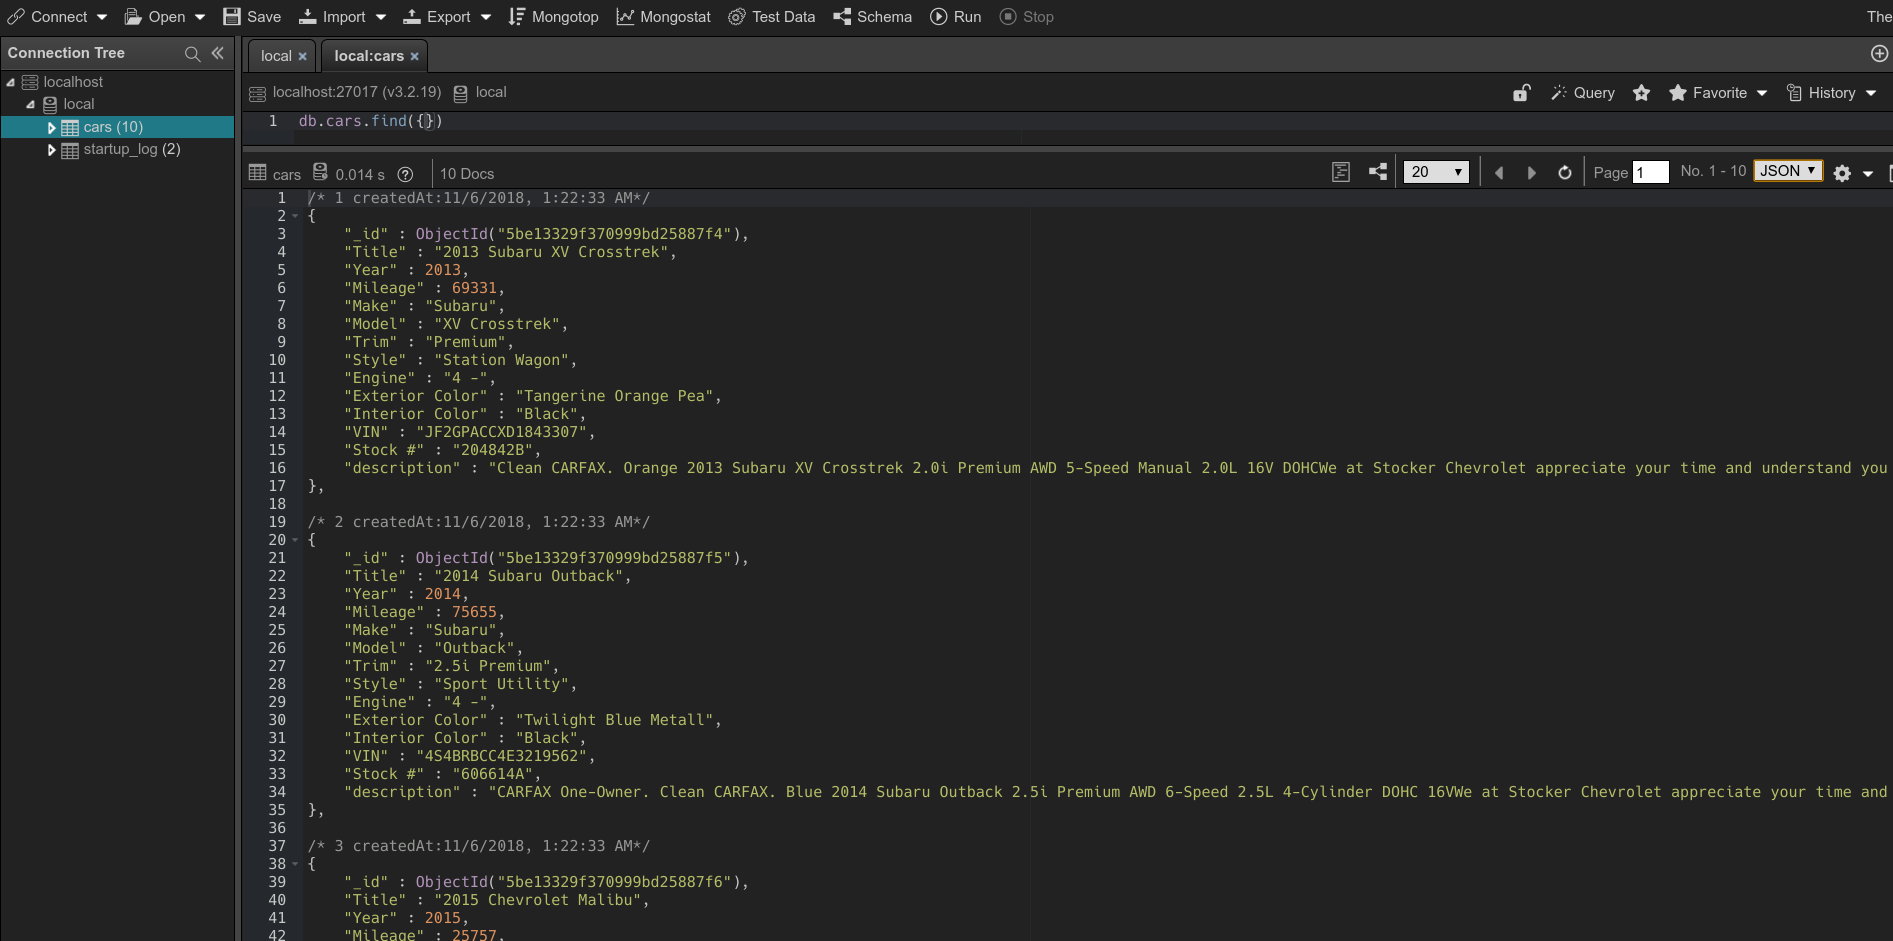
\includegraphics{1.png}
\caption{}
\end{figure}

    \subsection*{Task 2}\label{task-2}

Query your database and demonstrate that you can search on at least 2
attributes of the vehicles. Demonstrate a query on a single attribute
and a query on more than one attribute.

    \begin{itemize}
\item
  query on a single attribute
  
   \begin{figure}[H]
  	\centering
  	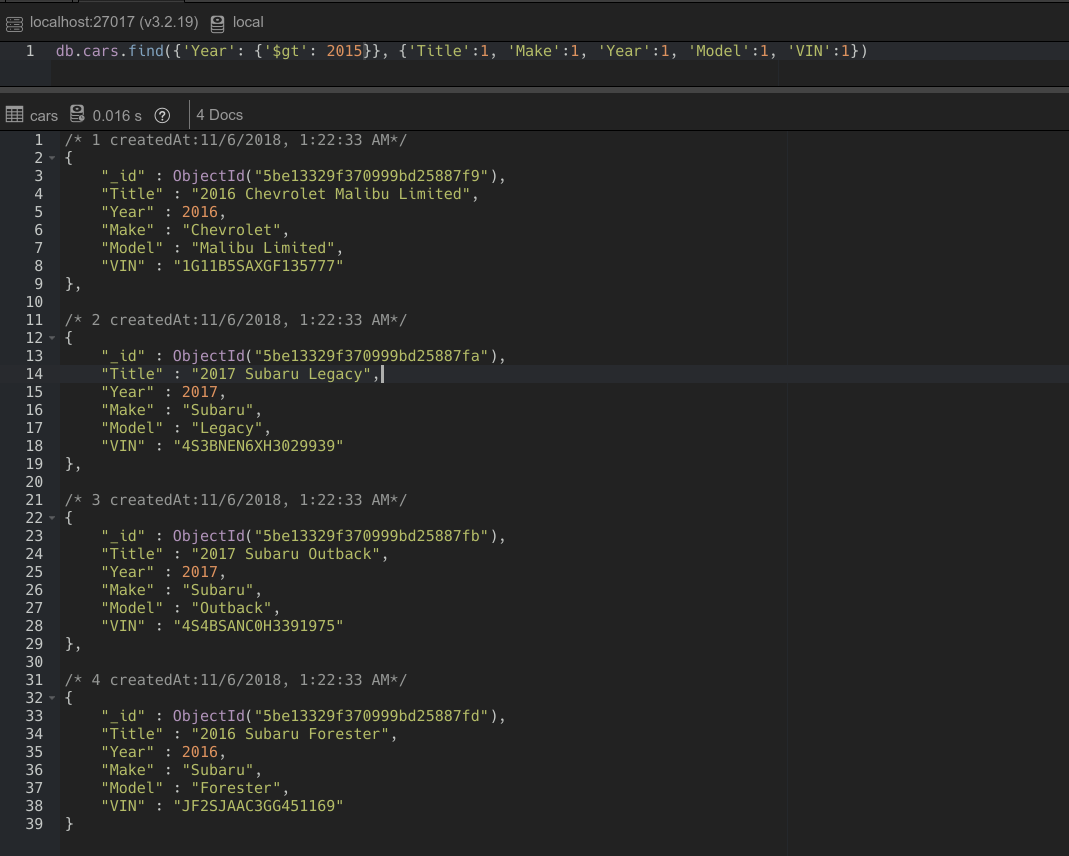
\includegraphics{2.png}
  	\caption{}
  \end{figure}
\item
  query on more than one attribute 
   \begin{figure}[H]
  	\centering
  	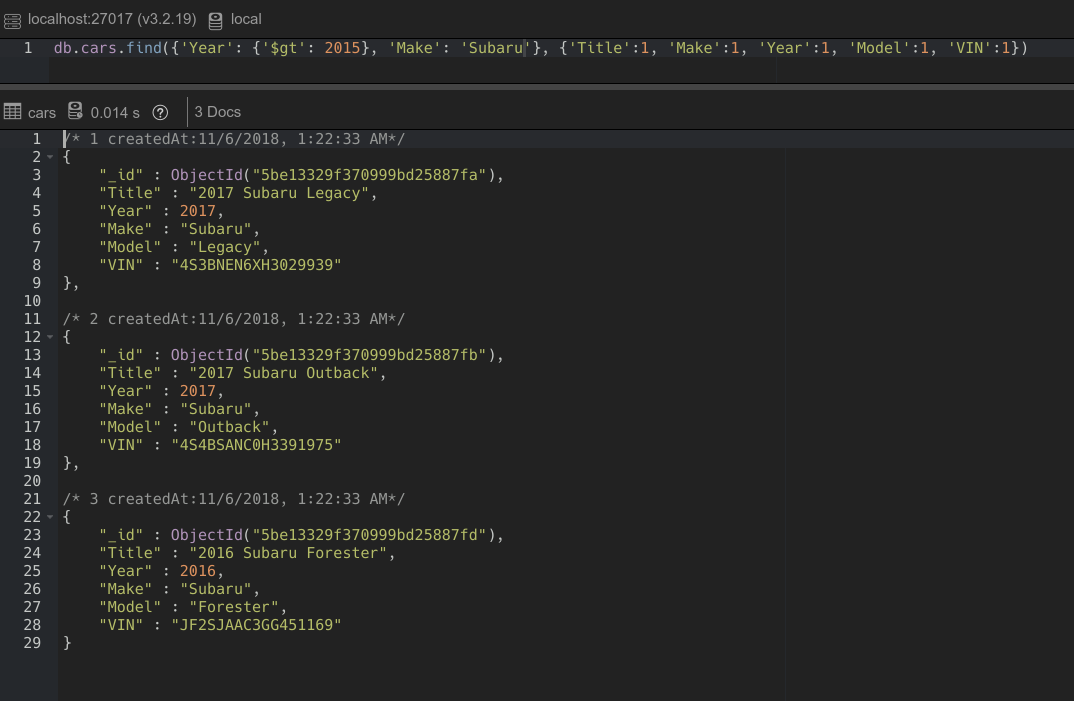
\includegraphics{3.png}
  	\caption{}
  \end{figure}
\end{itemize}

    \subsection*{Task 3}\label{task-3}

Demonstrate a query for a vehicle not in the database.

    \begin{figure}[H]
\centering
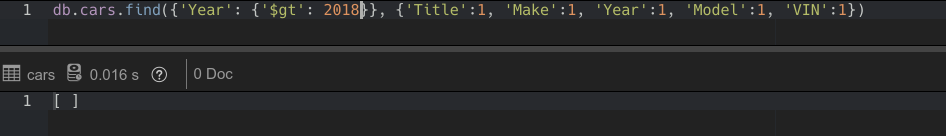
\includegraphics{4.png}
\caption{}
\end{figure}

It returns an empty set.

    \subsection*{Task 4}\label{task-4}

What are differences you found between using MongoDB and Redis for
loading and storing this data? What would be a role for a database like
Redis in storing this vehicle information? Can you imagine challenges in
using the method you used for data import into MongoDB when dealing with
Big Data? How might you address any challenges in a big data
environment?\\\\\

    With mongoDB we can import the whole dataset in the json format directly
while in Redis, we have to import one key-value pair at a time. In this
case, Redis acts like a dictionary in python used to store the nested
dictionaries (key-value pairs).

    \begin{itemize}
\tightlist
\item
  challenges:

  \begin{itemize}
  \tightlist
  \item
    the dataset to insert is too large
  \item
    take up too much memory
  \item
    it takes too long to import the whole dataset
  \end{itemize}
\item
  possible solutions to address the challenges:

  \begin{itemize}
  \tightlist
  \item
    import the data in batches

    \begin{itemize}
    \tightlist
    \item
      mongoimport -\/-db local -\/-collection cars -\/-file cars.json
      -\/-batchSize 1
    \end{itemize}
  \item
    disable journaling to avoid further memory consumption when tracking
    the changes made

    \begin{itemize}
    \tightlist
    \item
      mongod -\/-nojournal
    \end{itemize}
  \item
    import the dataset in parallel with \texttt{-\/-numInsertionWorkers}

    \begin{itemize}
    \tightlist
    \item
      mongoimport -\/-db local -\/-collection cars -\/-file cars.json
      -\/-numInsertionWorkers 8
    \end{itemize}
  \item
    convert text data into bson format
  \item
    use GridFS when the file exceeds the size limit of 16MB

    \begin{itemize}
    \tightlist
    \item
      mongofiles put cars.json
    \end{itemize}
  \item
    if there are complex analyses on the data involved before importing, such as applying a
    machine learning algorithm to do classification, a possible way is
    to use mongodb-spark-connector to analyze with spark mllib, then
    import dataset from hdfs back to mongodb:
  \end{itemize}
\end{itemize}

    \begin{Verbatim}[commandchars=\\\{\}]
{\color{incolor}In [{\color{incolor} }]:} \PY{n}{hdfs} \PY{n}{dfs} \PY{o}{\PYZhy{}}\PY{n}{put} \PY{n}{cars}\PY{o}{.}\PY{n}{csv} \PY{o}{/}\PY{n}{user}\PY{o}{/}\PY{n}{data}
        \PY{n}{pyspark} \PY{o}{\PYZhy{}}\PY{o}{\PYZhy{}}\PY{n}{packages} \PY{n}{org}\PY{o}{.}\PY{n}{mongodb}\PY{o}{.}\PY{n}{spark}\PY{p}{:}\PY{n}{mongo}\PY{o}{\PYZhy{}}\PY{n}{spark}\PY{o}{\PYZhy{}}\PY{n}{connector\PYZus{}2}\PY{o}{.}\PY{l+m+mi}{11}\PY{p}{:}\PY{l+m+mf}{2.2}\PY{o}{.}\PY{l+m+mi}{1}
                \PY{o}{\PYZhy{}}\PY{o}{\PYZhy{}}\PY{n}{packages} \PY{n}{org}\PY{o}{.}\PY{n}{mongodb}\PY{p}{:}\PY{n}{mongo}\PY{o}{\PYZhy{}}\PY{n}{java}\PY{o}{\PYZhy{}}\PY{n}{driver}\PY{p}{:}\PY{l+m+mf}{3.8}\PY{o}{.}\PY{l+m+mi}{0}
                \PY{o}{\PYZhy{}}\PY{o}{\PYZhy{}}\PY{n}{packages} \PY{n}{org}\PY{o}{.}\PY{n}{apache}\PY{o}{.}\PY{n}{spark}\PY{p}{:}\PY{n}{spark}\PY{o}{\PYZhy{}}\PY{n}{sql\PYZus{}2}\PY{o}{.}\PY{l+m+mi}{11}\PY{p}{:}\PY{l+m+mf}{2.3}\PY{o}{.}\PY{l+m+mi}{0}
                \PY{o}{\PYZhy{}}\PY{o}{\PYZhy{}}\PY{n}{packages} \PY{n}{com}\PY{o}{.}\PY{n}{stratio}\PY{o}{.}\PY{n}{datasource}\PY{p}{:}\PY{n}{spark}\PY{o}{\PYZhy{}}\PY{n}{mongodb\PYZus{}2}\PY{o}{.}\PY{l+m+mi}{11}\PY{p}{:}\PY{l+m+mf}{0.12}\PY{o}{.}\PY{l+m+mi}{0}
                \PY{o}{\PYZhy{}}\PY{o}{\PYZhy{}}\PY{n}{packages} \PY{n}{org}\PY{o}{.}\PY{n}{mongodb}\PY{p}{:}\PY{n}{casbah\PYZus{}2}\PY{o}{.}\PY{l+m+mi}{11}\PY{p}{:}\PY{l+m+mf}{3.0}\PY{o}{.}\PY{l+m+mi}{0}
                \PY{o}{\PYZhy{}}\PY{o}{\PYZhy{}}\PY{n}{packages} \PY{n}{org}\PY{o}{.}\PY{n}{apache}\PY{o}{.}\PY{n}{spark}\PY{p}{:}\PY{n}{spark}\PY{o}{\PYZhy{}}\PY{n}{catalyst\PYZus{}2}\PY{o}{.}\PY{l+m+mi}{11}\PY{p}{:}\PY{l+m+mf}{2.2}\PY{o}{.}\PY{l+m+mi}{1}
\end{Verbatim}

    \begin{Verbatim}[commandchars=\\\{\}]
{\color{incolor}In [{\color{incolor}1}]:} \PY{k+kn}{from} \PY{n+nn}{pyspark}\PY{n+nn}{.}\PY{n+nn}{sql} \PY{k}{import} \PY{n}{SparkSession}\PY{p}{,} \PY{n}{Row}\PY{p}{,} \PY{n}{functions}
        
        \PY{k}{def} \PY{n+nf}{parseInput}\PY{p}{(}\PY{n}{line}\PY{p}{)}\PY{p}{:}
            \PY{n}{fields} \PY{o}{=} \PY{n}{line}\PY{o}{.}\PY{n}{split}\PY{p}{(}\PY{l+s+s1}{\PYZsq{}}\PY{l+s+s1}{,}\PY{l+s+s1}{\PYZsq{}}\PY{p}{)}
            \PY{k}{return} \PY{n}{Row}\PY{p}{(}\PY{n}{Title} \PY{o}{=} \PY{n}{fields}\PY{p}{[}\PY{l+m+mi}{1}\PY{p}{]}\PY{p}{,} 
                       \PY{n}{Year} \PY{o}{=} \PY{n}{fields}\PY{p}{[}\PY{l+m+mi}{2}\PY{p}{]}\PY{p}{,}
                       \PY{n}{Mileage} \PY{o}{=} \PY{n}{fields}\PY{p}{[}\PY{l+m+mi}{3}\PY{p}{]}\PY{p}{,}
                       \PY{n}{Make} \PY{o}{=} \PY{n}{fields}\PY{p}{[}\PY{l+m+mi}{4}\PY{p}{]}\PY{p}{,}
                       \PY{n}{Model} \PY{o}{=} \PY{n}{fields}\PY{p}{[}\PY{l+m+mi}{5}\PY{p}{]}\PY{p}{,}
                       \PY{n}{Trim} \PY{o}{=} \PY{n}{fields}\PY{p}{[}\PY{l+m+mi}{6}\PY{p}{]}\PY{p}{,}
                       \PY{n}{Style} \PY{o}{=} \PY{n}{fields}\PY{p}{[}\PY{l+m+mi}{7}\PY{p}{]}\PY{p}{,}
                       \PY{n}{Engine} \PY{o}{=} \PY{n}{fields}\PY{p}{[}\PY{l+m+mi}{8}\PY{p}{]}\PY{p}{,}
                       \PY{n}{Exterior\PYZus{}Color} \PY{o}{=} \PY{n}{fields}\PY{p}{[}\PY{l+m+mi}{9}\PY{p}{]}\PY{p}{,}
                       \PY{n}{Interior\PYZus{}Color} \PY{o}{=} \PY{n}{fields}\PY{p}{[}\PY{l+m+mi}{10}\PY{p}{]}\PY{p}{,}
                       \PY{n}{VIN} \PY{o}{=} \PY{n}{fields}\PY{p}{[}\PY{l+m+mi}{11}\PY{p}{]}\PY{p}{,}
                       \PY{n}{Stock} \PY{o}{=} \PY{n}{fields}\PY{p}{[}\PY{l+m+mi}{12}\PY{p}{]}\PY{p}{,}
                       \PY{n}{description} \PY{o}{=} \PY{n}{fields}\PY{p}{[}\PY{l+m+mi}{13}\PY{p}{]}\PY{p}{)}
        
        \PY{k}{if} \PY{n+nv+vm}{\PYZus{}\PYZus{}name\PYZus{}\PYZus{}} \PY{o}{==} \PY{l+s+s1}{\PYZsq{}}\PY{l+s+s1}{\PYZus{}\PYZus{}main\PYZus{}\PYZus{}}\PY{l+s+s1}{\PYZsq{}}\PY{p}{:}
            \PY{n}{spark} \PY{o}{=} \PY{n}{SparkSession}\PY{o}{.}\PY{n}{builder}\PY{o}{.}\PY{n}{appName}\PY{p}{(}\PY{l+s+s1}{\PYZsq{}}\PY{l+s+s1}{MongoDBIntegration}\PY{l+s+s1}{\PYZsq{}}\PY{p}{)}\PY{o}{.}\PY{n}{getOrCreate}\PY{p}{(}\PY{p}{)}
            \PY{n}{lines} \PY{o}{=} \PY{n}{spark}\PY{o}{.}\PY{n}{sparkContext}\PY{o}{.}\PY{n}{textFile}\PY{p}{(}\PY{l+s+s1}{\PYZsq{}}\PY{l+s+s1}{hdfs://localhost:9002/user/data/cars.json}\PY{l+s+s1}{\PYZsq{}}\PY{p}{)}
            \PY{n}{cars} \PY{o}{=} \PY{n}{lines}\PY{o}{.}\PY{n}{map}\PY{p}{(}\PY{n}{parseInput}\PY{p}{)}
            \PY{n}{carsDataset} \PY{o}{=} \PY{n}{spark}\PY{o}{.}\PY{n}{createDataFrame}\PY{p}{(}\PY{n}{cars}\PY{p}{)}
            
            \PY{c+c1}{\PYZsh{} write into MongoDB}
            \PY{n}{carsDataset}\PY{o}{.}\PY{n}{write} \PYZbs{}
                        \PY{o}{.}\PY{n}{format}\PY{p}{(}\PY{l+s+s1}{\PYZsq{}}\PY{l+s+s1}{com.stratio.datasource.mongodb}\PY{l+s+s1}{\PYZsq{}}\PY{p}{)} \PYZbs{}
                        \PY{o}{.}\PY{n}{options}\PY{p}{(}\PY{n}{host}\PY{o}{=}\PY{l+s+s2}{\PYZdq{}}\PY{l+s+s2}{localhost:27017}\PY{l+s+s2}{\PYZdq{}}\PY{p}{,} \PY{n}{database}\PY{o}{=}\PY{l+s+s2}{\PYZdq{}}\PY{l+s+s2}{local}\PY{l+s+s2}{\PYZdq{}}\PY{p}{,} \PY{n}{collection}\PY{o}{=}\PY{l+s+s2}{\PYZdq{}}\PY{l+s+s2}{cars2}\PY{l+s+s2}{\PYZdq{}}\PY{p}{)} \PYZbs{}
                        \PY{o}{.}\PY{n}{mode}\PY{p}{(}\PY{l+s+s1}{\PYZsq{}}\PY{l+s+s1}{append}\PY{l+s+s1}{\PYZsq{}}\PY{p}{)} \PYZbs{}
                        \PY{o}{.}\PY{n}{save}\PY{p}{(}\PY{p}{)}
\end{Verbatim}

    \begin{figure}[H]
\centering
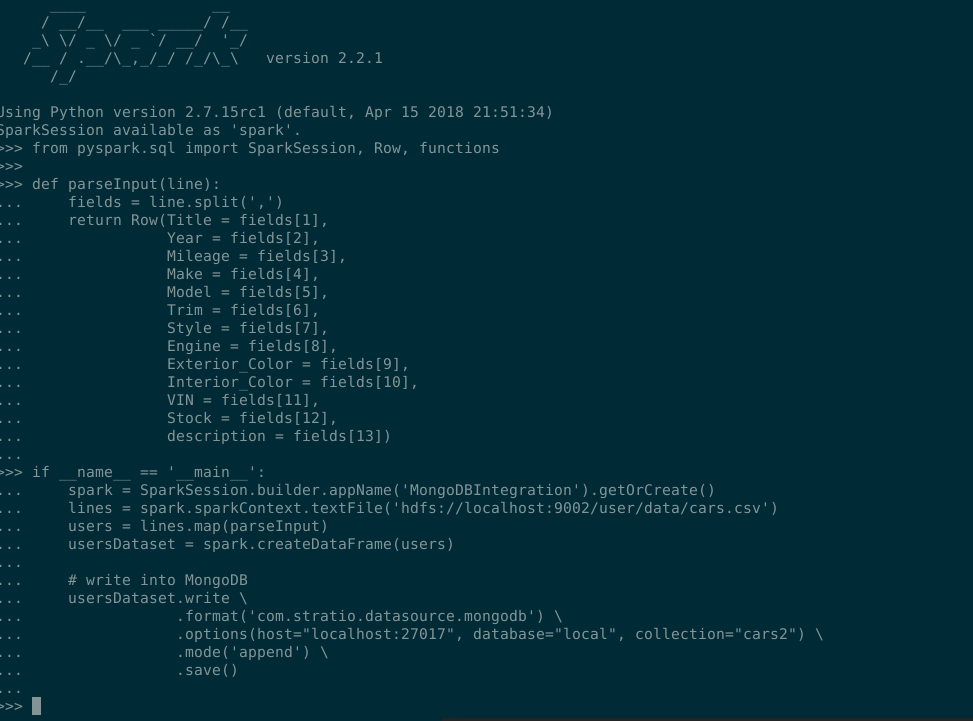
\includegraphics{6.png}
\caption{}
\end{figure}

\begin{figure}[H]
\centering
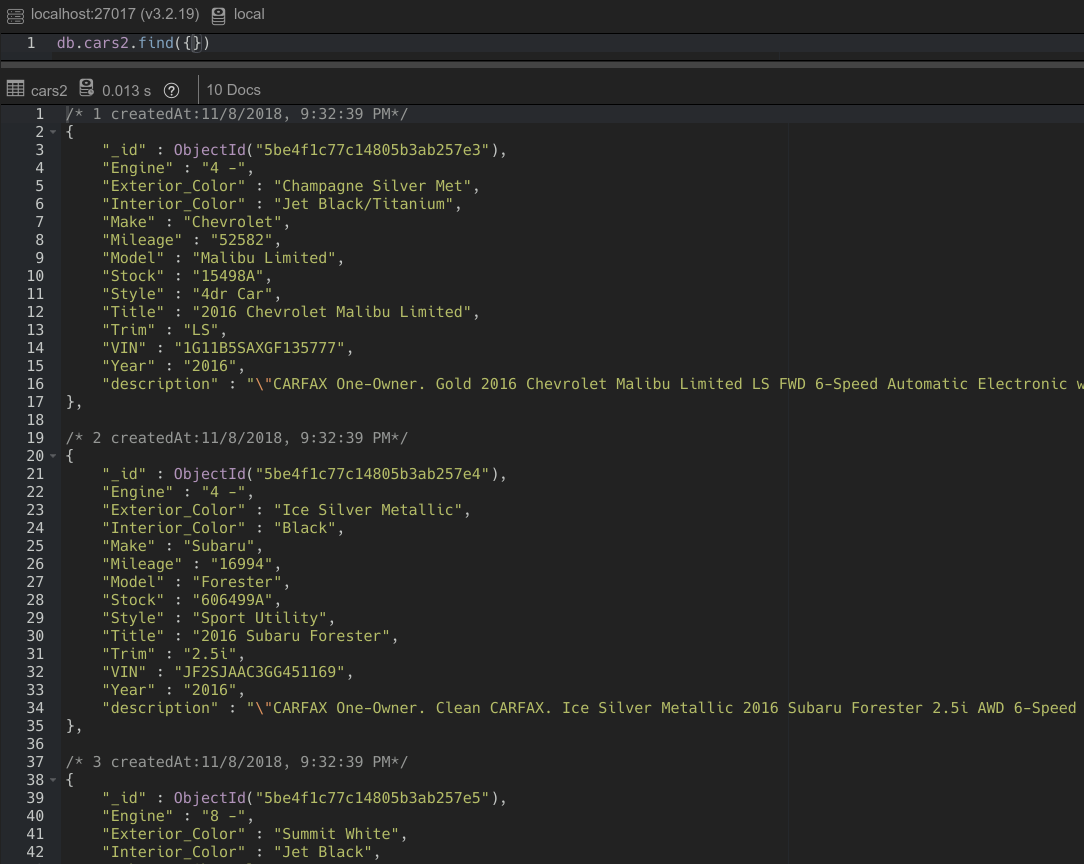
\includegraphics{7.png}
\caption{}
\end{figure}


    % Add a bibliography block to the postdoc
    
    
    
    \end{document}
